Trong những năm gần đây, sự phát triển của các hệ thống phần mềm đa luồng và thời gian thực đã làm gia tăng nhu cầu sử dụng các cơ chế đồng bộ hóa hiệu quả nhằm đảm bảo tính nhất quán dữ liệu và độ tin cậy của hệ thống. Trong các lĩnh vực như ô tô, hàng không và hệ thống nhúng, đối tượng \texttt{atomic} được sử dụng rộng rãi để hỗ trợ truy cập dữ liệu an toàn trong môi trường đồng thời mà không cần sử dụng cơ chế khóa truyền thống. Nhờ đó, chương trình có thể giảm chi phí đồng bộ hóa và cải thiện hiệu năng thực thi.

Tuy nhiên, việc kiểm thử các chương trình sử dụng \texttt{atomic} vẫn là một thách thức đối với nhiều công cụ kiểm thử hiện nay. Khác với các biến thông thường, đối tượng \texttt{atomic} cung cấp các thao tác chuyên biệt như \texttt{load}, \texttt{store}, \texttt{exchange} và \texttt{compare\_exchange}, đồng thời có ngữ nghĩa thực thi riêng liên quan đến cơ chế đồng bộ hóa. Điều này làm tăng độ phức tạp trong quá trình phân tích chương trình và xây dựng các ca kiểm thử phù hợp.

AKAUTAUTO là công cụ hỗ trợ kiểm thử đơn vị cho các dự án C/C++, được phát triển dựa trên kỹ thuật thực thi tượng trưng động. Công cụ đã hỗ trợ hiệu quả việc kiểm thử đối với nhiều kiểu dữ liệu thông thường. Tuy nhiên, hệ thống hiện chưa hỗ trợ đầy đủ các đối tượng \texttt{atomic}. Trong quá trình phân tích mã nguồn, các biến nguyên tử và các thao tác liên quan chưa được biểu diễn một cách phù hợp trong mô hình dữ liệu nội bộ, gây khó khăn cho việc xây dựng và thực thi các ca kiểm thử đối với các hàm sử dụng kiểu dữ liệu này.

% chktex-file 13
\begin{figure}[htbp]
    \centering
    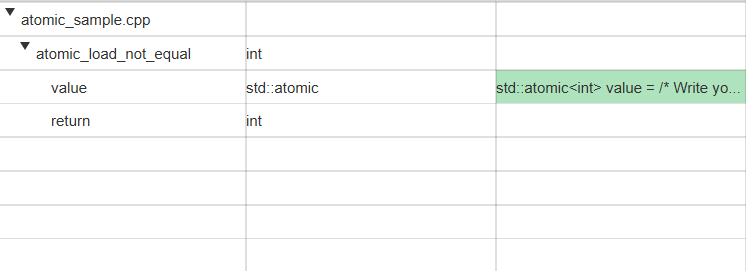
\includegraphics[width=0.9\textwidth]{images/atomic_begin.png}
    \caption{AKAUTAUTO chưa thể hiện được đúng trên Data Tree}
\end{figure}

Xuất phát từ thực trạng trên, báo cáo tập trung nghiên cứu và triển khai cơ chế hỗ trợ đối tượng \texttt{atomic} cho công cụ AKAUTAUTO. Các nội dung chính của đề tài bao gồm:

\begin{itemize}[leftmargin=*, itemsep=0.3em]
\item \textbf{Mở rộng mô hình dữ liệu:} Bổ sung cơ chế nhận diện và biểu diễn các đối tượng \texttt{atomic} trong quá trình phân tích cây cú pháp trừu tượng (AST).

\item \textbf{Hỗ trợ thực thi và đánh giá kiểm thử:} Cho phép người dùng khai báo giá trị kiểm thử cho các đối tượng \texttt{atomic}, thực thi chương trình và theo dõi kết quả độ phủ mã nguồn đối với các nhánh liên quan đến biến nguyên tử.

\end{itemize}

Kết quả đạt được góp phần mở rộng khả năng hỗ trợ của AKAUTAUTO đối với các chương trình sử dụng đối tượng \texttt{atomic}, tạo nền tảng cho việc nghiên cứu và phát triển các kỹ thuật sinh dữ liệu kiểm thử tự động cho môi trường đồng thời trong tương lai.
